

\subsection{Vista de Persona}
\label{sub:vista_persona}
Se creó una vista mediante la cual se pueda acceder a la información de cada persona y a la lista de actividades en las que se encuentra involucrada. Su
implementación se basó en la iteración de la colección de actividades  de la persona y la generación de html mediante \textbf{Twig}\@. Además,
se agregó estilo mediante \textbf{CSS} y una simple animación en \textbf{Javascript}.

\subsubsection{Introducción Twig}%
\label{ssub:introducción_twig}

Twig es el motor de \textit{templates} por defecto de \textbf{Symfony}, éste permite reutilizar elementos y agregar lógica a la vista en distintas partes de una aplicación web\@.


Un motor de \textit{templates} posibilita, entre otras cosas, reutilizar la estructura básica de una página y cambiar o sobrescribir aquello que varía.

Twig funciona mediante el uso de \textbf{bloques}, entendidos éstos como etiquetas que delimitan secciones del \textit{template}\@. Estas etiquetas tienen la función de indicarle al
motor de \textit{templates} que un \textit{template} \textit{hijo} puede sobrescribir estas partes del \textit{template}\@. De esta manera se consigue separar las partes estáticas
del sitio, de aquellas que son dinámicas.

\subsubsection{Estilo}%
\label{ssub:estilo}

Para la implementación del estilo de la vista, se utilizó \textbf{Sass}, un preprocesador del lenguaje de hojas de estilo CSS. El mismo permite, entre otras cosas, utilizar
funciones, variables y herencia de selectores. Se empleó en el desarrollo por el hecho de que al utilizar selectores anidados se simplifica
la lectura y comprensión de algunas partes de la implementación. Además, la opción de poder definir variables y funciones facilita mucho el desarrollo.


Se diseñó la distribución de elementos utilizando \textit{grid}, una característica de \textbf{CSS} que permite acomodar elementos en una cuadrícula\@.
En un principio, se decidió por asignar los elementos de acuerdo a la figura~\ref{fig:image/grid}. Esto significa que se separó el contenido en tres contenedores: el título
, la lista de actividades y los datos personales.

Se determinaron las reglas para distribuir los elementos de esta forma mediante CSS Grid:

\begin{lstlisting}[caption={Definición de filas y columnas de la cuadrícula.\\Fuente: Elaboración propia.}]
    display: grid;
    grid-template-columns: 1fr 1fr;
    grid-template-rows: 50px auto;
\end{lstlisting}

De esta manera, se establecieron dos columnas ocupando todo el espacio disponible y dos filas: una de 50px para el título y otra con un alto automático de manera que se ajuste a la
cantidad de actividades\@.  Una vez definida la cuadrícula, se estableció el espacio que utilizará cada contenedor.


\begin{lstlisting}[caption={Orientación del contenedor de actividad en la cuadrícula.\\Fuente: Elaboración propia.}]
.actividades{
    grid-column-start: 1;
    grid-column-end: 2;
    padding: 10px 20px;
}
\end{lstlisting}

\newpage
\begin{lstlisting}[caption={Orientación del contenedor del título de la accíon.\\Fuente: Elaboración propia.}]
.persona-header{
    grid-row-start: 1;
    grid-column-start: 1;
    grid-column-end: 2;
    h3{
        margin-left: 10px;
    }
}
\end{lstlisting}
\begin{lstlisting}[caption={Orientación del contenedor de datos personales.\\Fuente: Elaboración propia.}]
.datos-personales{
    grid-column-start: 2;
    grid-row-start: 1;
    grid-row-end: 3;
    padding: 20px;
}
\end{lstlisting}

\subsubsection{Template}%
\label{ssub:template}
En primer lugar, se comenzó heredando de un template general de \textbf{Sonata-Admin} denominado \textbf{standard\_layout} y se sobrescribió la sección o el bloque
\textbf{sonata\_admin\_content}, que es la parte en la cual se muestra el contenido de cada acción.



Dado que entre persona y actividad hay una relación de 1-n, cada \textit{objeto} \textbf{Persona} cuenta con una colección de actividades\@. Por lo tanto, se decidió definir
un contenedor para cada una, mediante la utilización de un bucle \textit{for} en \textbf{Twig}. Como resultado, se crea un contenedor y se insertan los datos por cada actividad
presente en la colección\@. El resultado de esta operación puede observarse en la figura~\ref{fig:image/vista_persona}\@.


Cada ítem de actividad está compuesto por un contenedor que actúa de \textit{header}, y otro que almacena los datos\@.




Se agregaron links en cada ítem de actividad, uno para visualizar la actividad y otro para modificarla, esto se logró obteniendo el nombre de la ruta desde una función en la
entidad y generando la ruta mediante la función \textit{path} que provee \textbf{Twig}\@. Además, se agregó un link que permite, mediante \textbf{Javascript}, expandir o colapsar
el contenedor de los datos de actividad\@.  Estos links se agregaron en el \textit{header} de cada actividad\@.

Cada actividad cuenta con un método en su entidad que comprueba si se encuentra activa o no. Este valor es utilizado en el template para dar indicación visual acerca del estado de la actividad\@.

\subsubsection{Obtención de rutas}%
\label{ssub:obtención_de_rutas}
En \textbf{Symfony}, el nombre de una ruta actúa de identificador de la misma\@. Si se desea generar una ruta, es necesario proveer como parámetro el nombre.


\textbf{Sonata} define sus rutas de la siguiente forma: \\

\textbf{admin\_app\_\{nombre\_de\_clase\}\_action} \\

Por ende, se optó por generar el nombre de la ruta a partir del nombre de la clase de la entidad. Esto quiere decir que, si se tiene una nombre de entidad igual a \textbf{Secretario}, mediante
operaciones de
manipulación de \textit{cadenas}, transformarla de \textbf{Secretario} a \textbf{admin\_app\_secretario\_acción}\@.  Para lograr esto, se creó un método en cada entidad, que permite obtener el nombre de
la ruta, a través del nombre de la clase.

\newpage
\begin{lstlisting}[caption={Obtención del nombre de una ruta.\\Fuente: Elaboración propia.}, label={lst:ruta}]
    public function getRoute()
    {
        $name = get_class($this);//$name=App\Entity\Rector
        $result = substr($name, 11);//$result=Rector
        $result = strtolower($result);//$result=rector
        $result = "admin_app_".$result."_";
        //$result=admin_app_rector_
        return [
            "id" => $this->getId(),
            "route" => $result
        ];
    }
\end{lstlisting}

Para generar una ruta desde un template, es necesario el nombre de la ruta y todos los parámetros que la misma requiera. En el caso del método del ejemplo~\ref{lst:ruta}, se necesita el id como parámetro.


\begin{lstlisting}[caption={Generación de una ruta desde un template.\\Fuente: Elaboración propia.}, label={lst:path}]
{{path(routeData.route ~ "edit", {id: routeData.id})}}
\end{lstlisting}


\begin{figure}[H]
    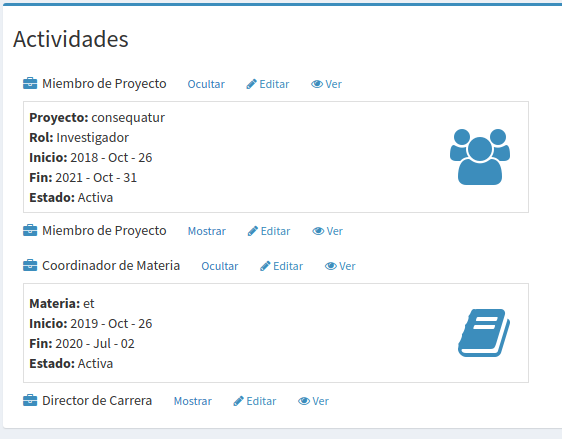
\includegraphics[width=1\linewidth]{image/vista_persona.png}
    \caption[Listado de actividades]{Listado de actividades.\newline \textbf{Fuente:} Elaboración propia, captura de pantalla de aplicación web.}
    \label{fig:image/vista_persona}
\end{figure}


\begin{figure}[h]
    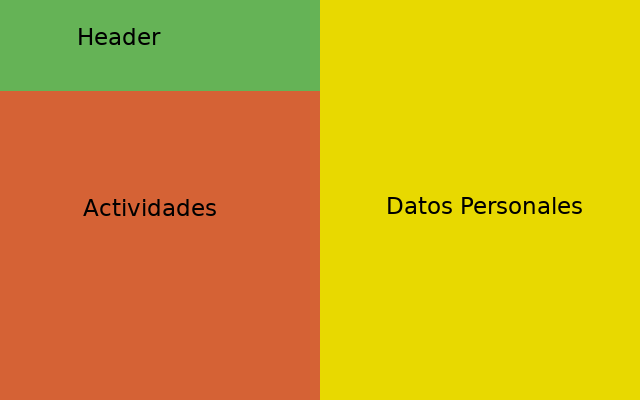
\includegraphics[width=1\linewidth]{image/grid.png}
    \caption[Distribución de columnas y filas]{Distribución de columnas y filas.\newline \textbf{Fuente:} Elaboración propia.}
    \label{fig:image/grid}
\end{figure}
